\subsection{Hybrid orbital representation}
\label{sec:spo_hybrid}
The hybrid representation of the single particle orbitals combines a localized atomic basis set around atomic cores and B-splines in the interstitial regions to reduce the memory usage while retaining high speed of evaluation and either retaining or increasing overall accuracy. Full details are provided in Ref.~\cite{Luo2018hyb}.
In practice, we have seen using meshfactor=0.5 is often possible and achieves huge memory saving.
Figure~\ref{fig:hybridrep} illustrates how the regions are assigned. Orbitals within region A are computed as
\[
  \phi^A_n({\bf r})=R_{n,l,m}(r)Y_{l,m}(\hat{r})
\]
Orbitals in region C are computed as the regular B-spline basis described in subsection~\ref{sec:spo_spline} above. The region B interpolates between A and C as
\begin{align}
  \phi^B_n({\bf r}) &= S(r) \phi^A_n({\bf r}) + (1-S(r))\phi^C_n({\bf r}) \\
                S(r) &= \frac{1}{2}-\frac{1}{2}\tanh\left[\alpha\left(\frac{r-r_{\rm A/B}}{r_{\rm B/C}-r_{\rm A/B}}-\frac{1}{2}\right)\right]
\end{align}

\begin{figure}
\centering
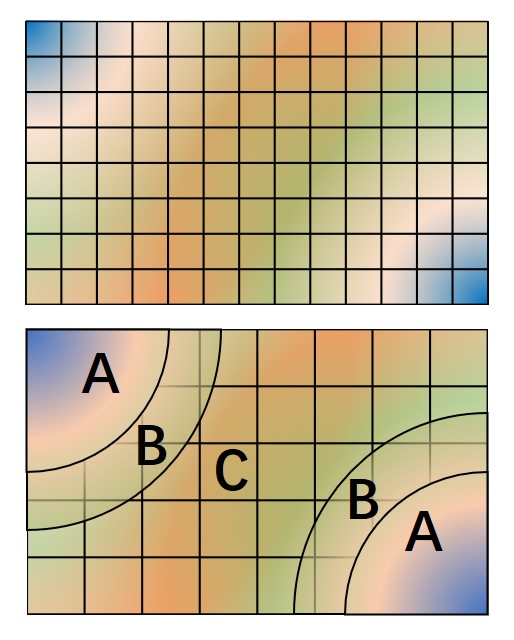
\includegraphics[trim={0 152 0 0},clip,width=0.45\columnwidth]{./figures/hybrid_new.jpg}
\qquad
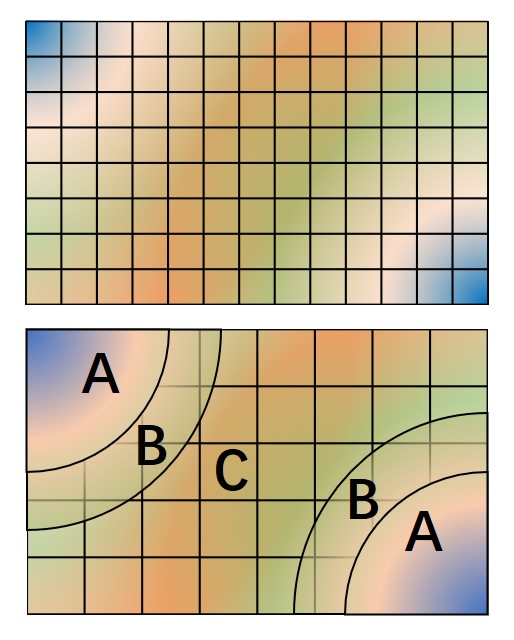
\includegraphics[trim={0 2 0 150},clip,width=0.45\columnwidth]{./figures/hybrid_new.jpg}
\caption{Illustration of regular and hybrid orbital representation. Regular B-spline representation (left panel) contains only one region and a sufficiently fine mesh to resolve orbitals near the nucleus. The hybrid orbital representation (right panel) contains near nucleus (A) regions where spherical harmonics and radial functions are used, buffers (B) or interpolation regions, and an interstitial (C) region where a coarse B-spline mesh is utilized.}
\label{fig:hybridrep}
\end{figure}

To enable hybrid orbital representation, the input XML needs to see the tag \texttt{hybridrep="yes"} shown below.
\begin{lstlisting}[caption=Hybrid orbital representation input example.\label{listing:hybridrep}]
<determinantset type="bspline" source="i" href="pwscf.h5"
                tilematrix="1 1 3 1 2 -1 -2 1 0" twistnum="-1" gpu="yes" meshfactor="0.8"
                twist="0  0  0" precision="single" hybridrep="yes">
  ...
</determinantset>
\end{lstlisting}
Second, the infomation describing the atomic regions is required in the particle set, shown below
\begin{lstlisting}[caption=particleset elements for ions with information needed by hybrid orbital representation.\label{listing:hybridrep_particleset}]
  <group name="Ni">
    <parameter name="charge">          18 </parameter>
    <parameter name="valence">         18 </parameter>
    <parameter name="atomicnumber" >   28 </parameter>
    <parameter name="cutoff_radius" > 1.6 </parameter>
    <parameter name="inner_cutoff" >  1.3 </parameter>
    <parameter name="lmax" >            5 </parameter>
    <parameter name="spline_radius" > 1.8 </parameter>
    <parameter name="spline_npoints">  91 </parameter>
  </group>
\end{lstlisting}

The parameters specific to hybrid representation are listed as
\begin{table}[h]
\centering
\begin{tabularx}{\textwidth}{l l l l l l }
\hline
\multicolumn{6}{l}{\texttt{attrib} element} \\
\hline
\multicolumn{2}{l}{attribute      :} & \multicolumn{4}{l}{}\\
   &   \bfseries name            & \bfseries datatype & \bfseries values & \bfseries default   & \bfseries description \\
   &   \texttt{cutoff\_radius}             &  real            &  $>=0.0$    &  \textit{none}    & The cutoff radius for B/C boundary  \\
   &   \texttt{lmax}         &  integer            &  $>=0$ &  \textit{none} & Largetst angular channel \\
   &   \texttt{inner\_cutoff}             &  real            &  $>=0.0$    &  dep.    & The cutoff radius for A/B boundary  \\
   &   \texttt{spline\_radius}         &  real            &  $>0.0$ &  dep. & radial function radius used in spline \\
   &   \texttt{spline\_npoints}         &  integer            &  $>0$ &  dep. & Number of spline knots \\
  \hline
\end{tabularx}
\end{table}

\begin{itemize}
  \item \texttt{cutoff\_radius} is required for every species. If a species is intended not being covered by atomic regions, setting the value 0.0 will put default values for all the reset parameters. A good value is usually a bit larger than the core radius listed in the pseudopotential file. After a parametric scan, pick the one from the flat energy region with the smallest variance.
  \item \texttt{lmax} is required if $\texttt{cutoff\_radius} > 0.0$. The value usually needs to be at least the highest angular momentum plus 2.
  \item \texttt{inner\_cutoff} is optional and set as $\texttt{cutoff\_radius}-0.3$ by default which is fine in most cases.
  \item \texttt{spline\_radius} and \texttt{spline\_npoints} are optional. By default, they are calculated based on \texttt{cutoff\_radius} and a grid distplacement $0.02$\,bohr.
        If users prefer inputing them, it is required that $\texttt{cutoff\_radius}<=\texttt{spline\_radius}-2\times\texttt{spline\_radius}/(\texttt{spline\_npoints}-1)$.
\end{itemize}

In addition, the hybrid orbital representation allows extra optimization to speed up the non-local pseudopotential evaluation using the batched algorithm listed in Sec.~\ref{sec:nlpp}.
